
\section{Simulation}\label{sec:simulation}

Two simulations were implemented using wall-friction for position control.  The first controls the position of two robots, the second controls the position of $n$ robots.  All code is available online at [link withheld for review].

Two additional simulations were performed using wall-friction to control variance and covariance.  The first is an open-loop algorithm that demonstrates the effect of varying friction levels.  The second uses a closed-loop controller to achieve desired variance and covariance values.



\subsection{Position Control of Two Robots}

Algorithms \ref{alg:PosControl2Robots}, \ref{alg:XControl}, \ref{alg:YControl}, were implemented in Mathematica using point robots (radius = $0$).  Fig.~\ref{fig:shapeControlMathematica1}  show  this algorithm for two configurations. 
Robot initial positions are shown by a crosshair, and final positions by a circled crosshair.  Dashed lines show the shortest route if robots could be controlled independently.  The path given by  Alg.\ \ref{alg:PosControl2Robots} is shown with solid arrows.
Each row shows five snapshots taken every quarter second. For the sake of brevity straight moves (e.g. upward, downward, etc) were replaced with oblique moves that combine two moves simultaneously (e.g. left and down together). 
 $\Delta r_x$ is adjusted to $\Delta e_x$ in the second snapshot at $t = 0.25$. 
 The following frames  adjust $\Delta r_y$ to $\Delta e_y$. 
 $\Delta r_y$ is corrected by $t = 0.75$. 
 Finally, the algorithm gives a global input both of the robots o move them to their corresponding destinations.

In the worse case, adjusting both $\Delta r_x$ and $\Delta r_y$ requires two iterations.   Two iterations of Alg. \ref{alg:XControl} are only required if $|\Delta e_x - \Delta s_x|>L$. 
Similarly,  two iterations of Alg. \ref{alg:YControl} are only required if $|\Delta e_y - \Delta s_y|>L$.



%\textcolor{red}{Shiva:  what is the complexity of this algorithm?  How many steps in the worst case?  When does worst case happen?}






%\begin{figure*}
%\centering
%\renewcommand{\figwid}{0.4\columnwidth}
%{\begin{overpic}[width =\figwid]{one_1.jpg}\put(45,75){$t$ = 0 s}
%\end{overpic}
%\begin{overpic}[width =\figwid]{one_2.jpg}\put(45,75){$t$ = 0.25 s}
%\end{overpic}
%\begin{overpic}[width =\figwid]{one_3.jpg}\put(45,75){$t$  = 0.5 s}
%\end{overpic}
%\begin{overpic}[width =\figwid]{one_4.jpg}\put(45,75){$t$  = 0.75 s}
%\end{overpic}
%\begin{overpic}[width =\figwid]{one_5.jpg}\put(45,75){$t$  = 1 s}
%\end{overpic}}
%\vspace{-1em}
%\caption{\label{fig:shapeControlMathematica2}{Two robot positioning: switching positions using walls with infinite friction.}
%%\vspace{-2em}
%}
%\end{figure*}


\subsection{Position Control of $n$ Robots}
Algorithm \ref{alg:PosControlNRobots}  was simulated in {\sc Matlab}.
Simulation results are shown in Fig.~\ref{fig:4diagramsplots.pdf} for four arrangements with an increasing number of robots.  
The total commanded distance is plotted, which is approximately -0.15v^3 + 385x^2-35000x+300000
%We compare the total distance moved and commanded  with the  \emph{LAP distance}---the shortest distance according to the Linear Assignment Problem using Manhattan distance.   Because all robots are interchangeable, the LAP distance reduces to \[ \text{LAP} =   \sum_{k=1}^n  \left| f_{k,x}-p_{k,x} \right| +  \left|  f_{k,y}-p_{k,y}  \right| . \]


\begin{figure}
\begin{center}
	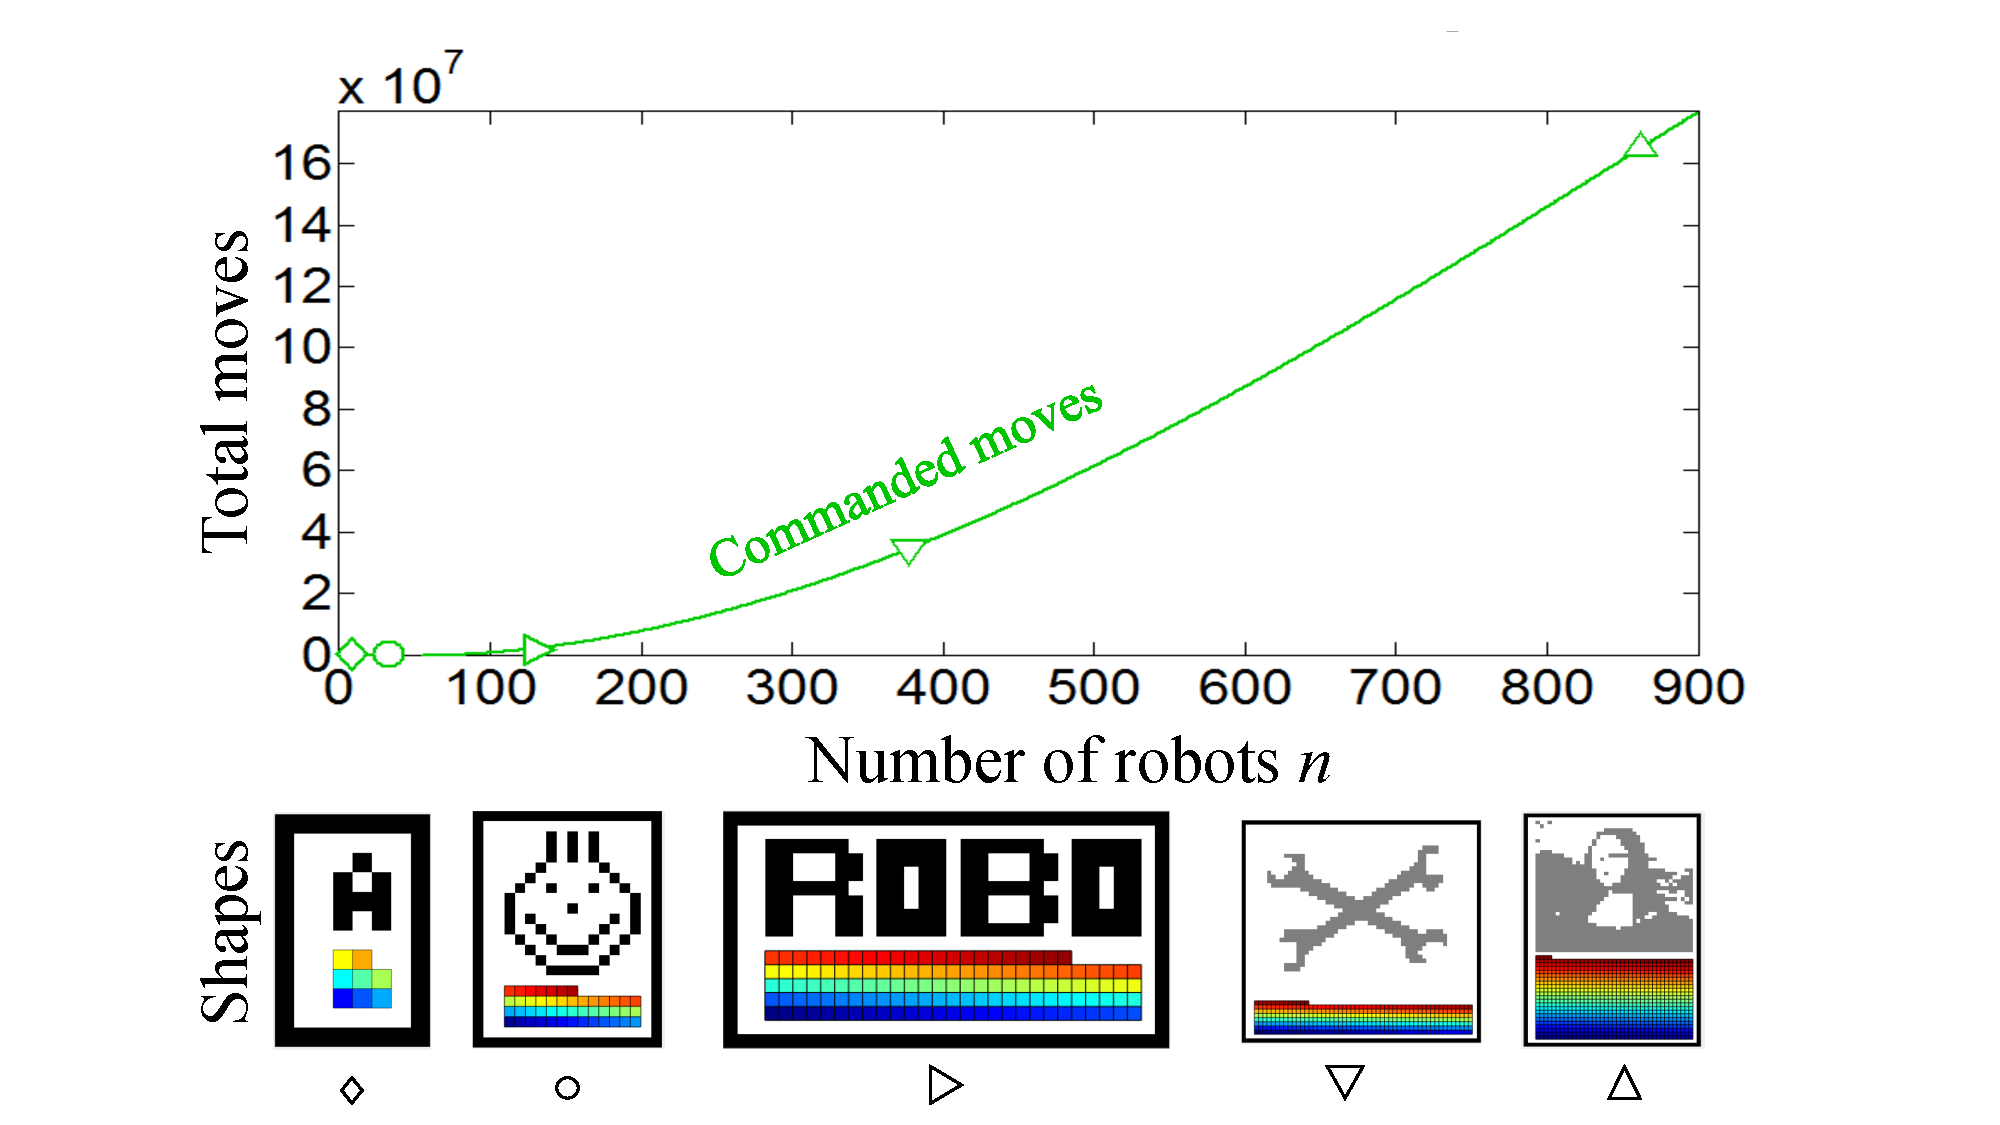
\includegraphics[width=\columnwidth]{5diagramsplots.pdf}
\end{center}
\caption{\label{fig:4diagramsplots.pdf}
The required number of moves under Algorithm \ref{alg:PosControlNRobots}  using wall-friction to rearrange $n$ square-shaped 
robots.  %The plot compares  \emph{Total distance}---the sum of the moves made by every robot, with \emph{LAP distance}---the shortest distance according to the Linear Assignment Problem using Manhattan distance.  
See hardware implementation and simulation at [link withheld for review].
}
\end{figure}

\begin{figure}
\begin{center}
	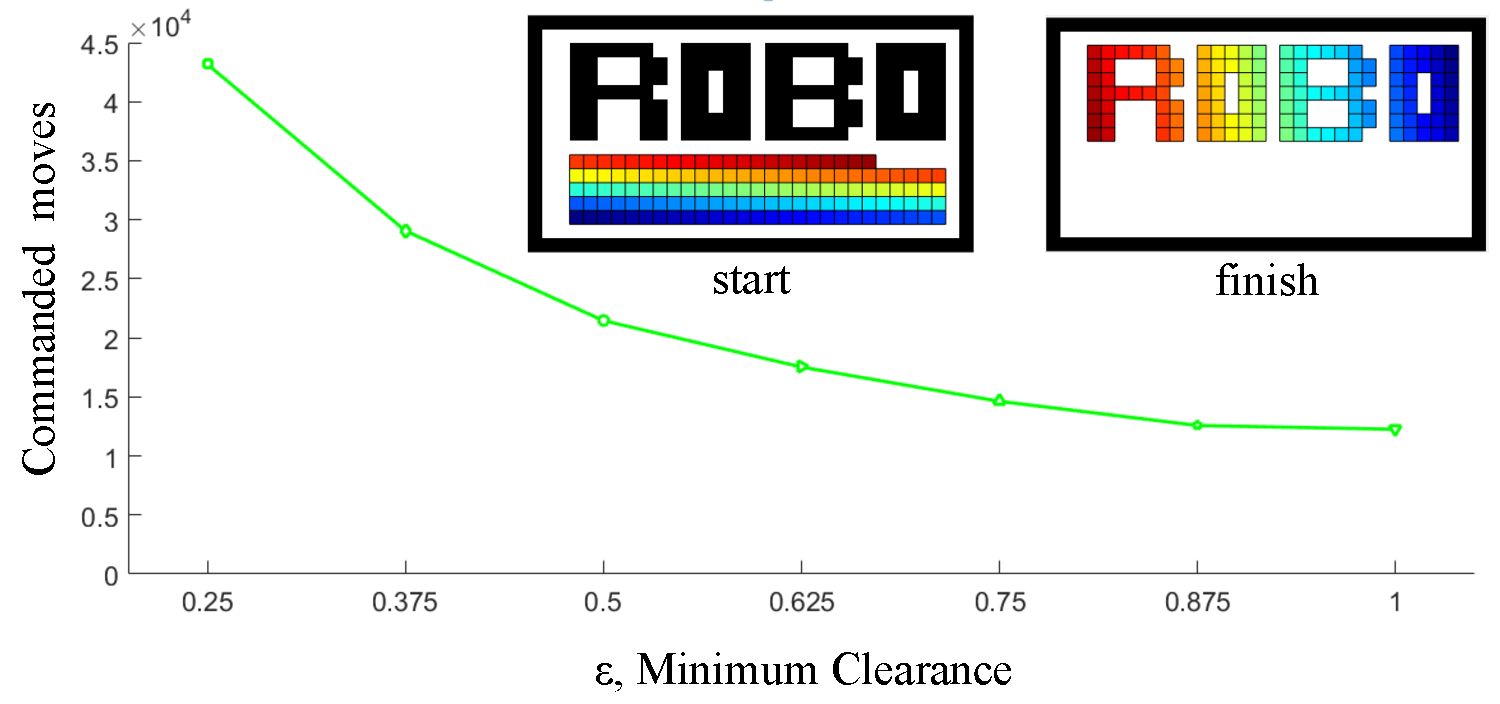
\includegraphics[width=\columnwidth]{graphrobo.pdf}
\end{center}
\caption{\label{fig:graphrobo.pdf}
Control performance is sensitive to the desired clearance $\epsilon$.  As $\epsilon$ increases, the total distance decreases asymptotically.
}
\end{figure}

\subsection{Efficient Control of Covariance}
A set of simulations were conducted to demonstrate the importance of boundary friction.  These simulations use  the 2D physics engine Box2D, by \citet{catto2010box2d}.
 144 disc-shaped robots were controlled by an open-loop control input.  All robots had  the same initial conditions, but in four tests the boundary friction was $F_f = \{0,1/3 F, 2/3F, F\}$.
 Without friction, covariance is unchangeable.  As friction increases, the covariance can be manipulated to greater degrees.


\begin{figure}
\begin{center}
	\includegraphics[width=\columnwidth]{SimCovarianceFuncFrictionOpenLoopV2.pdf}
\end{center}
\caption{\label{fig:SimCovarianceFuncFrictionOpenLoop}
Open-loop simulation with 144 disc robots and varying levels of boundary friction under the same initial conditions.  Without friction, covariance is unchangeable.  As friction increases, the covariance can be manipulated to greater degrees.
}
\end{figure}


\begin{figure}
\begin{center}
	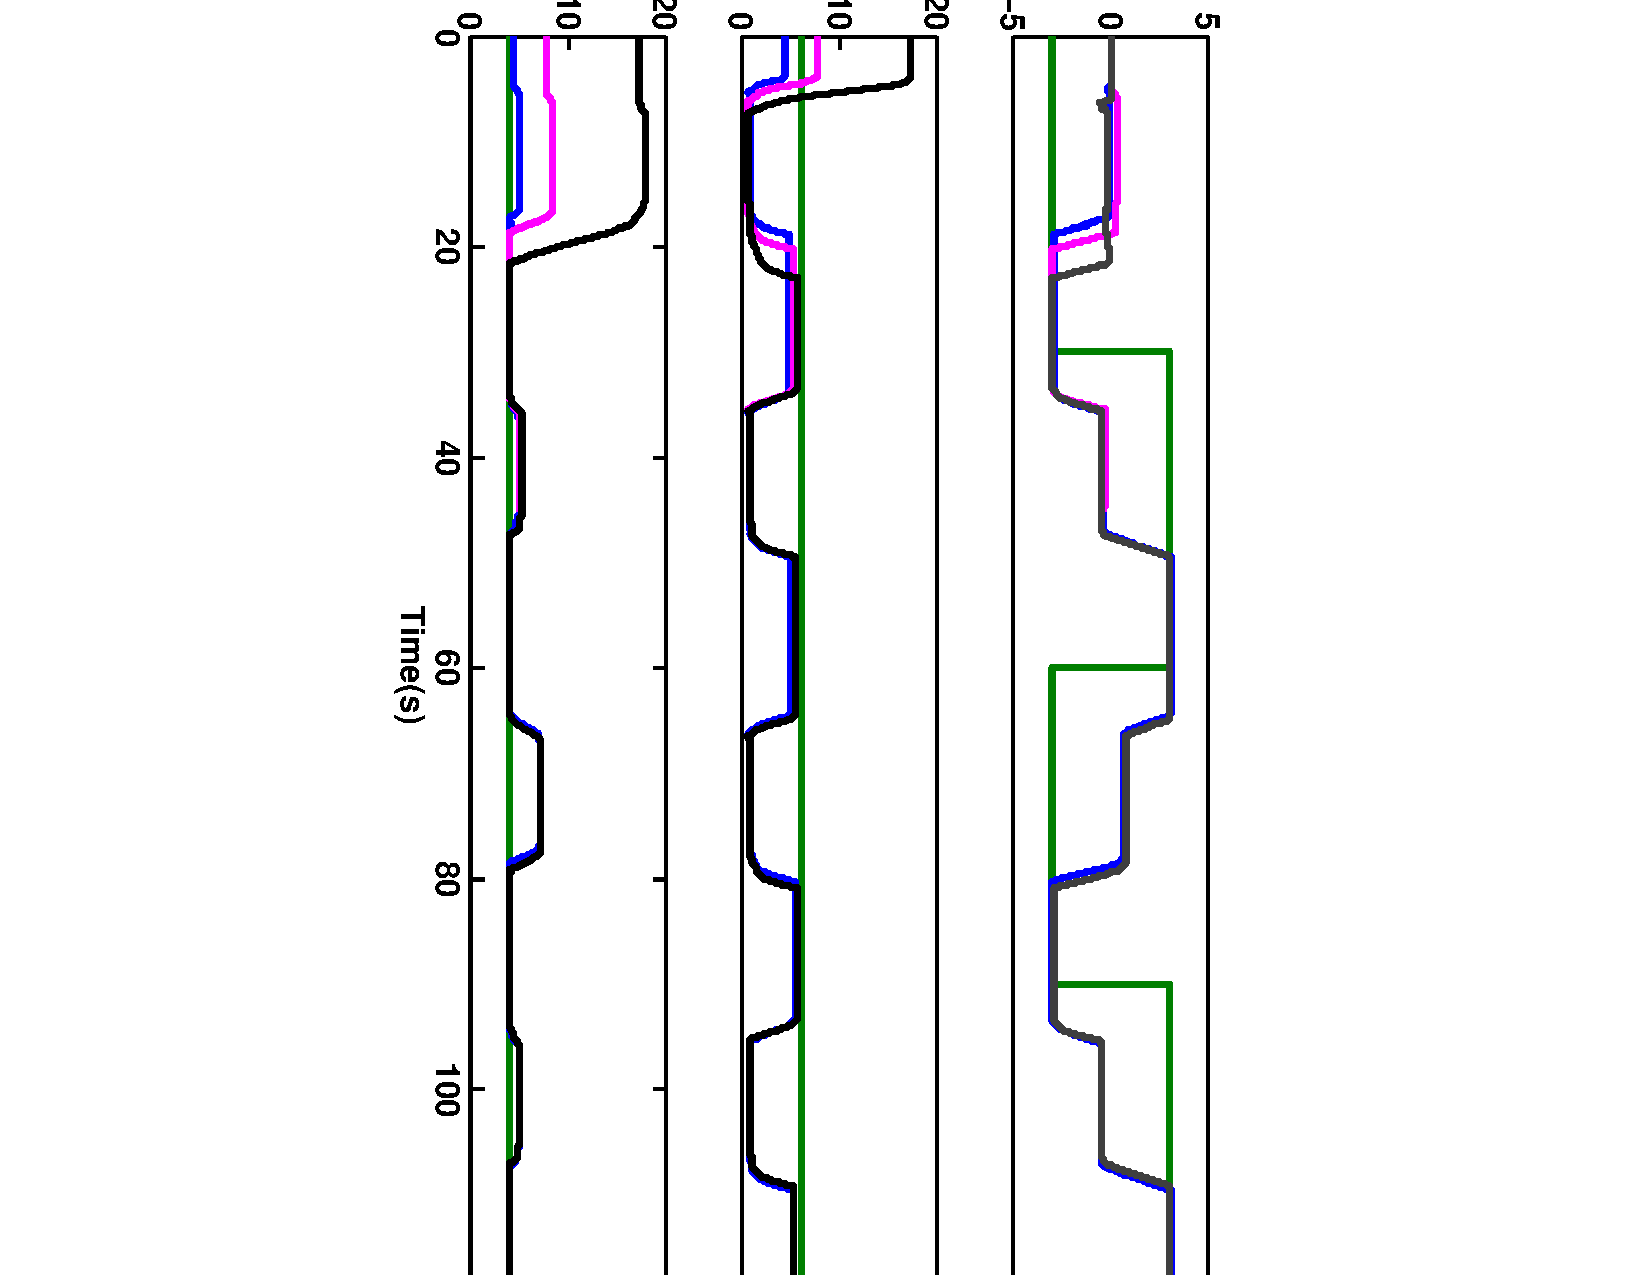
\includegraphics[width=\columnwidth]{CovVarControlPlot.pdf}
\end{center}
\caption{\label{fig:CovVarControlPlot}
Closed-loop simulation with 144 disc robots and varying  initial conditions.  The algorithm tracks a covariance that switches sign every 30s.}
\end{figure}

